\chapter{Manipulação de Dados no Jamovi}

O foco deste capítulo é a manipulação de dados, uma habilidade essencial para qualquer pessoa que esteja interessada em análise de dados. Vamos explorar as diversas funções e recursos do Jamovi para tratar, organizar e manipular conjuntos de dados. Se você já se perguntou como criar e gerenciar categorias, transformar dados ou manipular variáveis no Jamovi, este capítulo irá te guiar através desses processos passo a passo.

No capítulo anterior você deu os primeiros passos e apresentamos a você a interface do Jamovi para manipulação de dados. Nesse capítulo discutiremos o fluxo de trabalho ideal para o tratamento de um conjunto de dados. O objetivo é garantir que você tenha uma compreensão sólida das ferramentas disponíveis e de como usá-las eficientemente.

Em seguida, abordaremos como criar novas categorias a partir de variáveis existentes. Isso pode ser útil em uma variedade de contextos, como quando você deseja agrupar respostas de pesquisas ou classificar dados em grupos específicos. Também ensinaremos a transformar variáveis, permitindo que você mude o formato dos seus dados de uma maneira que melhor atenda às suas necessidades analíticas.

Finalmente, traremos exemplos práticos para aplicar o conhecimento adquirido. O intuito é promover a familiarização com as ferramentas do software e reforçar a compreensão das funcionalidades abordadas.

Lembre-se, a manipulação eficaz dos dados é a base de qualquer análise de qualidade. Por isso, este capítulo desempenha um papel fundamental no seu aprendizado sobre o uso do Jamovi. Esperamos que ao final desta etapa, você se sinta confiante para manipular conjuntos de dados e prepará-los para a análise de uma maneira eficiente e eficaz.

\section{Introdução à Manipulação de Dados}
Nesta seção, apresentaremos o papel crucial da manipulação de dados na análise de dados. Exploraremos seu propósito, benefícios e relevância no contexto do software Jamovi.

Deixe-me contar algo importante antes de começarmos a falar sobre análises estatísticas complexas. Sabe aquele momento em que você recebe um conjunto de dados e se pergunta "por onde começo"? Pois é, antes de criar aqueles gráficos impressionantes ou realizar testes estatísticos sofisticados, existe uma etapa fundamental que muitas vezes passa despercebida: a manipulação de dados.

Quando eu comecei a trabalhar com análise de dados, confesso que subestimava essa etapa. Achava que era apenas uma questão de abrir a planilha e começar a analisar. Mas rapidamente aprendi que dados do mundo real raramente vêm organizados e prontos para uso. Eles chegam com erros de digitação, valores faltantes, formatos inconsistentes e tantos outros problemas que, se não tratados adequadamente, podem comprometer toda a análise posterior.

A manipulação de dados é como preparar o terreno antes de construir uma casa. Sem uma base sólida, todo o resto fica comprometido. Ela envolve desde a limpeza básica (corrigir erros, eliminar duplicatas), passando pela transformação de variáveis (converter formatos, criar novas variáveis a partir das existentes), até filtragem, agregação e reestruturação dos dados. Parece trabalhoso? Sim, pode ser. Mas acredite, este investimento inicial economiza horas de frustração mais tarde.

O Jamovi, felizmente, nos ajuda bastante nessa jornada. Ele oferece várias ferramentas que facilitam a manipulação básica e intermediária dos dados. Você pode criar e transformar variáveis, recodificar valores, filtrar observações, tratar dados ausentes e muito mais, tudo através de uma interface amigável que não exige conhecimentos avançados de programação.

No entanto, é importante que você saiba que, como qualquer software, o Jamovi tem suas limitações. Quando trabalhamos com conjuntos de dados muito grandes ou precisamos fazer operações de reestruturação complexas, podemos enfrentar alguns desafios. O software pode ficar lento ao processar milhares de observações, e algumas técnicas avançadas de limpeza de dados não estão disponíveis nativamente.

Por isso, em muitos dos meus projetos, acabo utilizando uma abordagem híbrida. Uso o Excel ou Google Sheets para algumas limpezas iniciais e organização básica, principalmente quando preciso fazer verificações visuais rápidas ou ajustes em massa. Para manipulações mais complexas, recorro ocasionalmente ao R ou Python, especialmente em projetos maiores. Só então importo os dados para o Jamovi para a análise estatística final.

Não se preocupe se você não tem experiência com essas outras ferramentas. O Jamovi é perfeitamente capaz de lidar com a maioria das situações que você encontrará, especialmente em contextos acadêmicos e pesquisas de pequeno a médio porte. E neste capítulo, vou compartilhar com você algumas dicas e truques que aprendi ao longo dos anos para contornar as limitações do software.

O mais importante é entender que a manipulação de dados não é apenas uma etapa técnica, mas uma parte fundamental do processo analítico que influencia diretamente a qualidade dos seus resultados. Quanto mais limpos e bem organizados estiverem seus dados, mais confiáveis serão suas análises e conclusões.

Nas próximas páginas, vamos explorar juntos como realizar essas tarefas no Jamovi, com exemplos práticos e orientações passo a passo. Meu objetivo é que, ao final deste capítulo, você se sinta confiante para transformar aqueles dados brutos e desorganizados em um conjunto pronto para revelar seus segredos através da análise estatística.

\section{Interface do Jamovi}

Antes de mergulharmos nas análises estatísticas, é fundamental conhecermos bem a interface do Jamovi. Uma compreensão clara da organização do programa nos permitirá navegar com eficiência e aproveitar todo seu potencial.

Ao abrir o Jamovi pela primeira vez, você se deparará com uma tela dividida em duas áreas principais :

\begin{itemize}
    \item \textbf{Área de Dados (esquerda):} Nesta região ficam exibidas todas as variáveis do seu conjunto de dados, similar a uma planilha. Aqui você visualizará, criará e modificará suas variáveis.

    \item \textbf{Área de Resultados (direita):} É a seção onde serão exibidos todos os outputs das análises, como tabelas, gráficos e estatísticas. Esta área, inicialmente identificada pelo logotipo do Jamovi sobre fundo branco, será preenchida conforme você executa análises.
\end{itemize}

Na parte superior da interface, encontramos a barra de ferramentas principal com quatro menus essenciais:

\begin{itemize}
    \item \textbf{Menu Arquivo:} Localizado no extremo superior esquerdo, permite criar um novo banco de dados, abrir arquivos existentes, importar dados de outros formatos, salvar seu trabalho e exportar resultados. Logo abaixo deste menu, você encontrará um histórico dos arquivos recentemente abertos, facilitando o acesso rápido a projetos em andamento.

    \item \textbf{Menu Variáveis:} Oferece opções para criar novas variáveis, adicionar descrições (conhecidas como ``labels'' em outros softwares estatísticos), transformar variáveis existentes e gerenciar seus metadados (Figura \ref{fig:interface_jamovi_1}).

    \item \textbf{Menu Dados:} Concentra as funcionalidades relacionadas à manipulação do conjunto de dados como um todo, permitindo transformações, cálculos, adição ou remoção de casos, entre outras operações.

    \item \textbf{Menu Análises:} Possivelmente o mais utilizado, contém todas as ferramentas estatísticas disponíveis no programa, desde análises descritivas básicas (frequências, medidas de tendência central) até testes mais avançados como regressão, ANOVA e testes não-paramétricos.
\end{itemize}

\begin{figure}[H]
    \centering
    \caption{Visão geral da interface do Jamovi, mostrando as áreas de dados e resultados}
    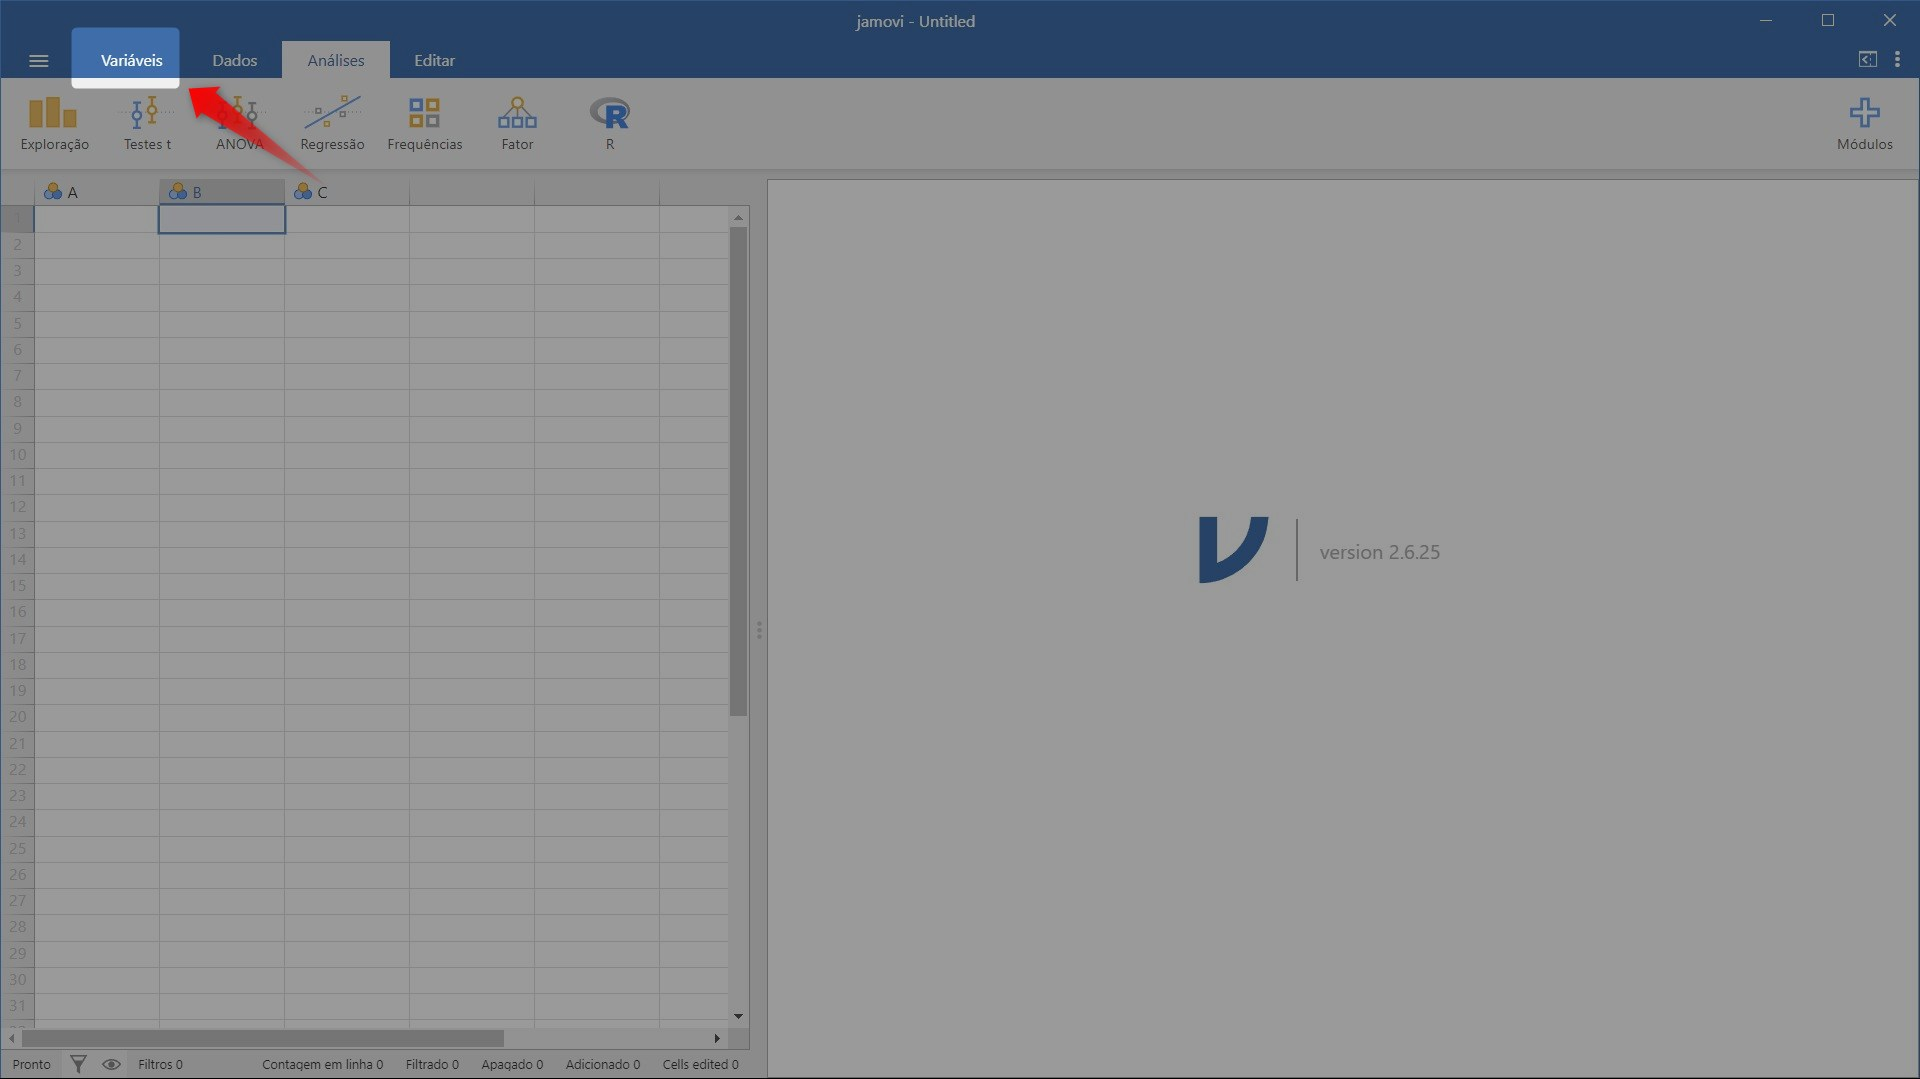
\includegraphics[width=\textwidth]{imagens/cap_2/interface_jamovi_1.jpg}
    \label{fig:interface_jamovi_1}
\end{figure}

Um diferencial interessante do Jamovi é seu \textbf{Editor de Resultados}, acessível através do menu ``Editar''. Esta funcionalidade transforma a área de resultados em um documento editável, semelhante a um relatório técnico. Você pode adicionar textos explicativos, títulos formatados, links e até fórmulas matemáticas entre suas análises. Por exemplo, é possível inserir a famosa equação $E=mc^2$ usando a função de fórmulas, criar cabeçalhos para seções do seu relatório, ou adicionar textos em itálico para destacar conceitos importantes.

Esta capacidade de documentação integrada elimina a necessidade de exportar resultados para outro software antes de elaborar seu relatório final, tornando seu fluxo de trabalho mais eficiente.

O design do Jamovi prioriza a simplicidade sem sacrificar a funcionalidade. Embora a interface possa parecer minimalista à primeira vista, ela contém todas as ferramentas necessárias para análises estatísticas robustas. Como veremos ao longo desta apostila, o Jamovi consegue ser simultaneamente acessível para iniciantes e poderoso para usuários avançados.

À medida que nos aprofundarmos em cada funcionalidade nas próximas seções, recomendo que você explore a interface por conta própria. Familiarizar-se com a localização das ferramentas agora facilitará significativamente seu trabalho quando começarmos a realizar análises estatísticas propriamente ditas.

\begin{tcolorbox}[colback=white,colframe=red,title={\faPlayCircle \ Dica de Conteúdo}]
  Preparei um vídeo apresentando a Interface do Jamovi, que vai te ajudar a dar os primeiros passos nessa incrível ferramenta estatística. Depois de ler a seção da apostila, não deixe de conferir essa videoaula, tenho certeza de que você vai adorar e aprender muito. Clique no link abaixo e aproveite!\\
  \textcolor{red}{\faYoutube} \href{https://youtu.be/bV9hlHPLe5I?si=h43c1jAG01oxltOB}{Jamovi - Interface do Jamovi}
\end{tcolorbox}

\section{Importação de Dados}

A importação de dados é um dos primeiros passos fundamentais para começar a trabalhar com análises estatísticas no Jamovi. O software oferece uma interface simples e intuitiva para este processo, permitindo importar dados de diversas fontes e formatos.

\subsection{Preparação dos dados antes da importação}

Antes de iniciar a importação propriamente dita, é fundamental realizar uma preparação prévia dos seus dados. Esta etapa, muitas vezes negligenciada, pode poupar tempo e evitar problemas durante as análises subsequentes:

\begin{itemize}
    \item \textbf{Limpe seus dados em uma planilha}: Abra seus dados em softwares como Excel ou Google Sheets antes de importá-los para o Jamovi.
    \item \textbf{Remova células mescladas}: Arquivos com células mescladas frequentemente causam problemas durante a importação.
    \item \textbf{Trate valores ausentes}: Identifique e padronize como os dados ausentes estão representados.
    \item \textbf{Verifique a consistência}: Certifique-se de que as variáveis estão no formato adequado (numérico, texto, data).
    \item \textbf{Salve em formato compatível}: Preferencialmente, salve os dados em formato CSV para garantir melhor compatibilidade.
\end{itemize}

Esta preparação prévia é especialmente importante quando trabalhamos com dados de fontes oficiais, como IBGE, que frequentemente vêm com formatações específicas que podem dificultar a importação direta.

\subsection{Processo de importação no Jamovi}

O processo de importação de dados no Jamovi é bastante simples e direto:

\begin{enumerate}
    \item Abra o Jamovi e clique no botão \textbf{Abrir} localizado no canto superior esquerdo da interface.
    \item Na janela que se abre, você verá duas opções principais:
    \begin{itemize}
        \item \textbf{Este PC}: Para importar arquivos salvos no seu computador.
        \item \textbf{Biblioteca de dados}: Para acessar conjuntos de dados já incluídos no Jamovi.
    \end{itemize}
    \item Para importar dados externos, selecione \textbf{Este PC}.
    \item Navegue até a pasta onde seu arquivo está armazenado, ou use o botão \textbf{Procurar} para localizar o arquivo.
    \item Selecione o arquivo desejado e clique em \textbf{Abrir}.
    \item O Jamovi importará os dados automaticamente, realizando configurações iniciais baseadas nos tipos de dados detectados.
    \item Verifique se a importação ocorreu corretamente, confirmando se todas as variáveis e observações estão presentes e no formato adequado.
\end{enumerate}

\begin{figure}[H]
    \centering
    \caption{Importando dados no Jamovi através do menu Arquivo}
    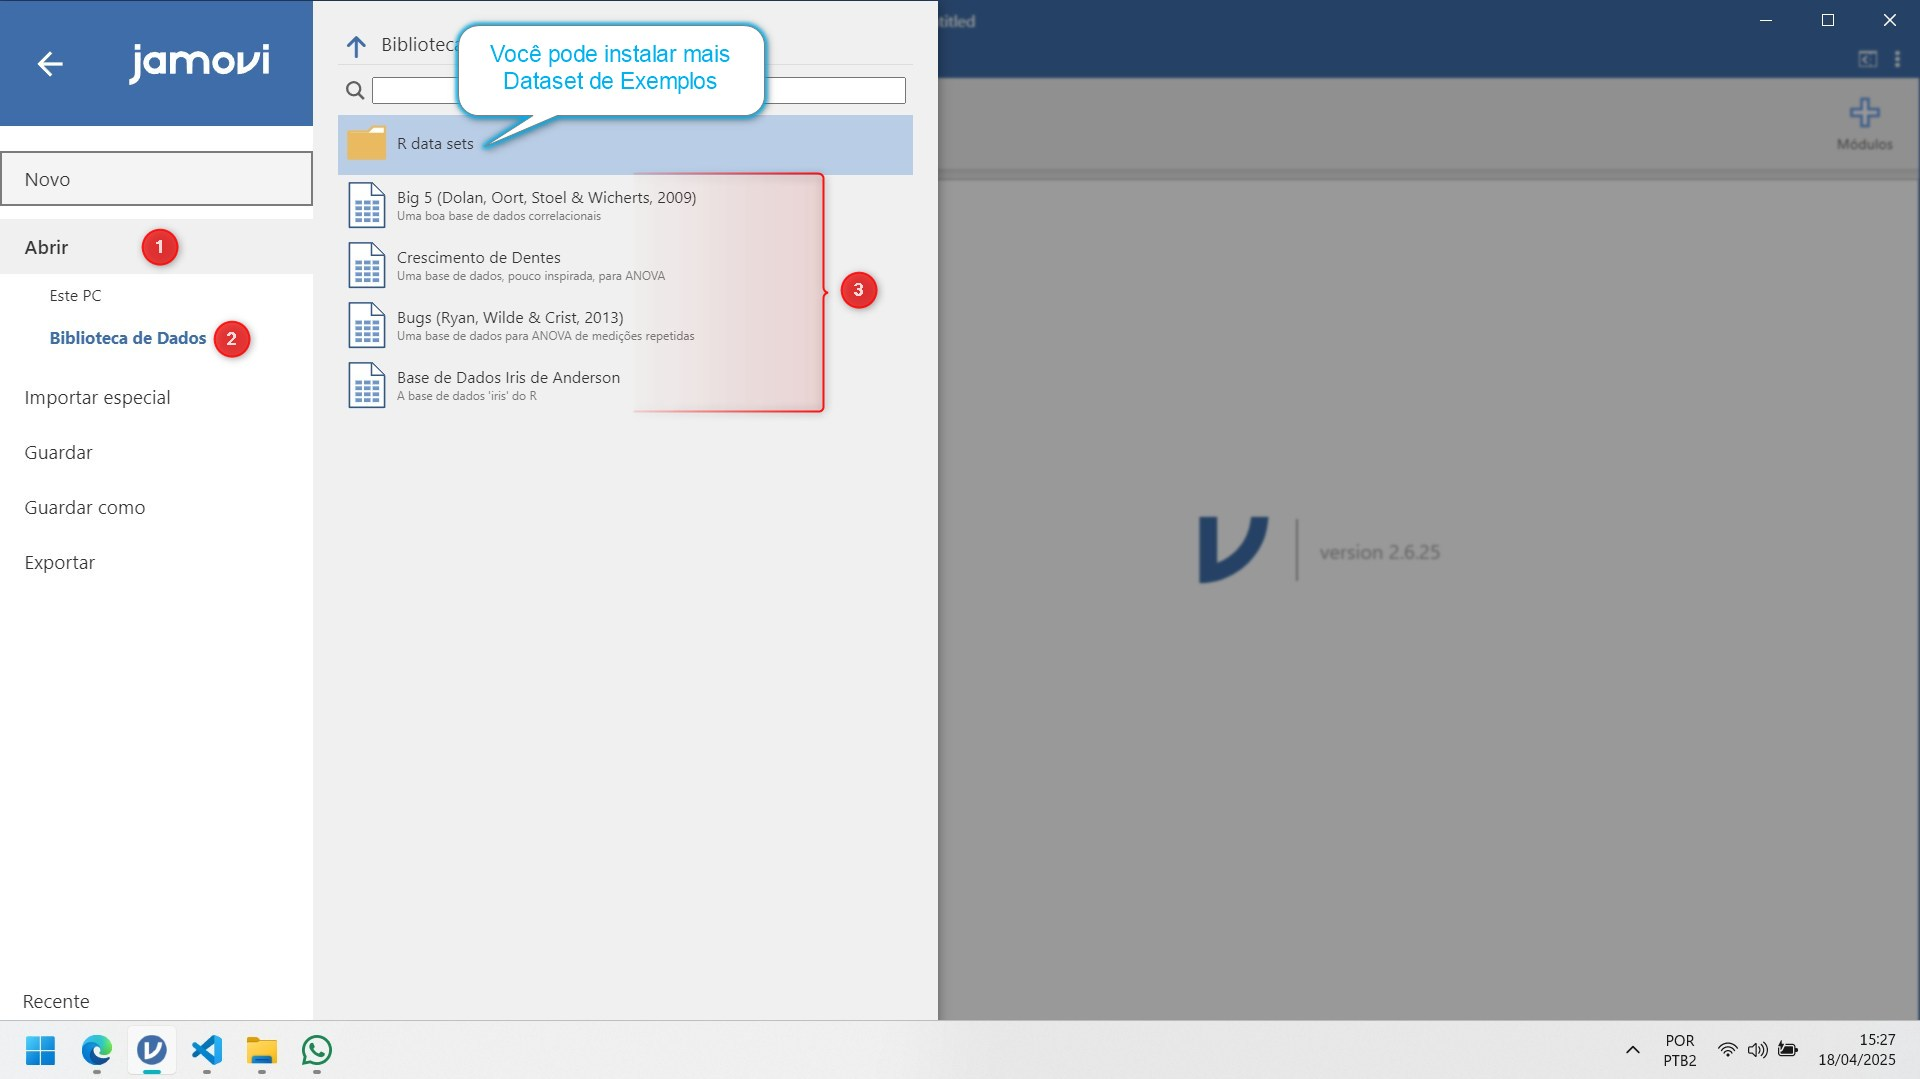
\includegraphics[width=\textwidth]{imagens/cap_2/importar_dados_jamovi_1.jpg}
    \label{fig:importar_dados_jamovi_1}
\end{figure}

\subsection{Biblioteca de dados integrada}

O Jamovi inclui uma biblioteca de conjuntos de dados pré-carregados que podem ser úteis para prática e ensino:

\begin{itemize}
    \item Na tela de abertura de arquivos, selecione \textbf{Biblioteca de dados}.
    \item Você encontrará diversos conjuntos clássicos, como o dataset Iris de Anderson, frequentemente usado em cursos introdutórios de estatística.
    \item Estes dados são particularmente úteis para professores e estudantes que desejam praticar técnicas estatísticas sem precisar coletar ou importar dados externos.
\end{itemize}

\subsection{Formatos de arquivo suportados}

O Jamovi suporta diversos formatos de arquivo, incluindo:

\begin{itemize}
    \item CSV (Comma-Separated Values)
    \item Excel (.xlsx, .xls)
    \item Arquivos de texto (.txt)
    \item Arquivos SPSS (.sav)
    \item Arquivos SAS (.sas7bdat)
    \item Arquivos Stata (.dta)
    \item Arquivos R (.rdata, .rds)
    \item Arquivos do próprio Jamovi (.omv)
\end{itemize}

Entre esses formatos, o CSV é geralmente recomendado por sua simplicidade e compatibilidade universal, minimizando problemas de importação.

\begin{tcolorbox}[colback=white,colframe=red,title={\faPlayCircle \ Dica de Conteúdo}]
  Para ver este processo em ação, confira meu tutorial em vídeo sobre importação de dados no Jamovi. O vídeo demonstra passo a passo como importar diferentes tipos de arquivos e resolver problemas comuns de importação.\\
  \textcolor{red}{\faYoutube} \href{https://youtu.be/NIpt0wIq5pc?si=IjYrrMqUSNfltmJ9}{Importação de Dados no Jamovi}
\end{tcolorbox}

\section{Inserir variável no Jamovi}

Embora o Jamovi seja principalmente usado para analisar dados já existentes, às vezes precisamos adicionar novas variáveis diretamente no software. Nesta seção, aprenderemos como inserir novas variáveis no Jamovi e adicionar dados manualmente.

\subsection{Quando inserir variáveis diretamente no Jamovi}

Antes de aprendermos o processo de inserção de variáveis, é importante considerar quando é apropriado fazê-lo:

\begin{itemize}
    \item \textbf{Pequenas adições}: Quando precisamos adicionar uma ou poucas variáveis a um conjunto de dados já importado.
    \item \textbf{Variáveis calculadas}: Quando precisamos criar uma variável que é resultado de cálculos baseados em outras variáveis.
    \item \textbf{Categorização}: Quando desejamos criar uma variável categórica a partir de dados existentes.
    \item \textbf{Protótipos}: Para criar pequenos conjuntos de dados para testes ou demonstrações.
\end{itemize}

No entanto, é importante ressaltar que para conjuntos de dados grandes ou completos, é geralmente mais eficiente preparar os dados em planilhas como Excel ou Google Sheets antes de importá-los para o Jamovi.

\subsection{Adicionando uma nova variável}

O processo para adicionar uma nova variável no Jamovi é bastante simples:

\begin{enumerate}
    \item Clique no menu \textbf{Variáveis} na barra superior.
    \item Selecione a opção \textbf{Adicionar}.
    \item Na janela que aparece, selecione \textbf{Acrescentar} para adicionar uma nova coluna ao final da tabela.
    \item Uma nova variável será adicionada com um nome padrão (geralmente "var").
\end{enumerate}

Alternativamente, você pode:
\begin{enumerate}
    \item Clicar com o botão direito do mouse em qualquer cabeçalho de variável.
    \item Selecionar a opção \textbf{Adicionar Variável} no menu de contexto.
\end{enumerate}

% \begin{figure}[H]
%     \centering
%     \caption{Adicionando uma nova variável no Jamovi}
%     \includegraphics[width=\textwidth]{imagens/cap_2/inserir_variavel_1.jpg}
%     \label{fig:inserir_variavel_1}
% \end{figure}

\subsection{Nomeando e configurando a variável}

Após adicionar a variável, é importante configurá-la adequadamente:

\begin{enumerate}
    \item Clique no nome padrão da variável para editá-lo.
    \item Atribua um nome seguindo as boas práticas de nomenclatura:
    \begin{itemize}
        \item Use nomes curtos e descritivos.
        \item Evite espaços (use underscore ``\_'' se necessário);
        \item Não use acentos ou caracteres especiais.
        \item Prefira letras minúsculas.
        \item Não inicie com números.
        \item Mantenha um padrão de nomenclatura.
    \end{itemize}
    \item Adicione uma descrição à variável no campo apropriado.
    \item Configure o tipo de medida (nominal, ordinal ou contínua) conforme necessário.
\end{enumerate}

Estas boas práticas de nomenclatura são particularmente importantes se você planeja exportar seus dados para outros softwares como R ou Python no futuro, pois evitam problemas de compatibilidade.

% \begin{figure}[H]
%     \centering
%     \caption{Nomeando e configurando uma variável no Jamovi}
%     \includegraphics[width=\textwidth]{imagens/cap_2/inserir_variavel_2.jpg}
%     \label{fig:inserir_variavel_2}
% \end{figure}

\subsection{Inserindo dados manualmente}

Para inserir dados na nova variável:

\begin{enumerate}
    \item Clique duas vezes na célula onde deseja inserir o dado.
    \item Digite o valor desejado.
    \item Pressione Enter ou clique em outra célula para confirmar.
    \item Continue preenchendo as demais células conforme necessário.
\end{enumerate}

\subsection{Apagando variáveis}

Se precisar remover uma variável, existem duas maneiras de fazê-lo:

\begin{enumerate}
    \item \textbf{Método 1:} 
    \begin{itemize}
        \item Clique no menu \textbf{Variáveis}.
        \item Selecione a variável que deseja apagar.
        \item Clique no botão \textbf{Apagar}.
    \end{itemize}
    
    \item \textbf{Método 2:}
    \begin{itemize}
        \item Clique com o botão direito no cabeçalho da variável.
        \item Selecione a opção \textbf{Apagar Variável}.
    \end{itemize}
\end{enumerate}

Para apagar múltiplas variáveis de uma vez:
\begin{enumerate}
    \item Mantenha a tecla Shift pressionada e clique nos cabeçalhos das variáveis que deseja selecionar.
    \item Clique com o botão direito em uma das variáveis selecionadas.
    \item Escolha a opção \textbf{Apagar Variável}.
\end{enumerate}

\begin{tcolorbox}[colback=white,colframe=red,title={\faPlayCircle \ Dica de Conteúdo}]
  Para ver na prática como inserir e gerenciar variáveis no Jamovi, confira meu tutorial em vídeo. Nele, mostro passo a passo como adicionar, configurar e remover variáveis, além de dicas úteis para uma melhor organização dos seus dados.\\
  \textcolor{red}{\faYoutube} \href{https://youtu.be/UqEnetiHEns?si=qvTd5AucIA88QR3j}{Como Inserir Variáveis no Jamovi}
\end{tcolorbox}


\section{Transformação de Variáveis}
A transformação de variáveis é um aspecto essencial da manipulação de dados. Aqui, exploraremos as diferentes maneiras de transformar variáveis no Jamovi.

\section{Criação de Categorias}
Nessa seção, discutiremos como criar e gerenciar categorias no Jamovi. Isso é particularmente útil ao lidar com variáveis categóricas e dados de pesquisa.

Para ilustrar como isso é feito, usaremos o Dataset de População - IBGE como exemplo. Este dataset contém dados sobre a população dos municípios brasileiros, com informações coletadas nos censos de 2010 e 2022, bem como projeções populacionais realizadas pelo IBGE. Os dados de população são especialmente adequados para a criação de categorias, já que podem ser agrupados de várias maneiras.

Neste tutorial, iremos focar em como usar esse dataset para criar categorias populacionais que representam cidades grandes, médias e pequenas. Este é um exemplo comum de como os dados populacionais são categorizados para análises demográficas, urbanísticas ou sociais.

Para começar, precisamos definir quais são os critérios para uma cidade ser considerada grande, média ou pequena. Essa definição pode variar dependendo do contexto, mas para os fins deste tutorial, iremos definir as categorias da seguinte forma: cidades pequenas são aquelas com população inferior a 20.000 habitantes, cidades médias possuem entre 20.000 e 100.000 habitantes, e cidades grandes são aquelas com mais de 100.000 habitantes.\footnote{Por favor, note que essa classificação é puramente ilustrativa e serve apenas para o propósito deste tutorial. Essa divisão de categorias não possui uma base científica rigorosa e pode variar consideravelmente dependendo do contexto específico. É importante ressaltar que, em sua própria análise, você está livre para definir suas próprias categorias com base nos critérios que considerar mais relevantes para o seu estudo.}

Após a importação dos dados, o primeiro passo para criar categorias no Jamovi é utilizar a opção "Transformar Variáveis". Existem duas maneiras de acessar essa funcionalidade.

A primeira maneira é através do menu de dados. Clique no menu "Dados" na parte superior da interface do Jamovi. Em seguida, selecione a opção "Transformar". Neste ponto, você pode selecionar a variável que deseja transformar em categorias.

A segunda opção, que é um pouco mais direta, envolve clicar com o botão direito do mouse no cabeçalho da variável que você deseja transformar. No menu que aparecerá, selecione a opção "Transformar".

Essas ações são ilustradas na Figura~\ref{fig:criar_categoria_jamovi}. Essa figura indica onde você precisa clicar para acessar a opção de transformação de variáveis.

Por favor, note que a escolha do método para acessar a opção de transformação de variáveis depende da sua preferência. Ambos os métodos levam ao mesmo resultado, então você pode escolher o que achar mais conveniente.

\begin{figure}[H]
    \centering
    \caption{Selecionando a Opção Transformar no Jamovi}
    \includegraphics[width=\textwidth]{imagens/cap_2/criar_categoria_jamovi.png}
    \label{fig:criar_categoria_jamovi}
\end{figure}

No exemplo que vamos tratar neste tutorial, estaremos utilizando a variável \textit{pop\_ibge\_2022}. Esta variável refere-se à população dos municípios brasileiros conforme estimado no censo do IBGE de 2022. Esta variável contínua será transformada em uma variável categórica que representa cidades grandes, médias e pequenas, de acordo com os critérios de classificação que definimos anteriormente.

Agora, precisamos configurar a nova variável categórica que será criada. Nesta etapa, você deverá escolher um nome para a nova variável. No nosso exemplo, chamaremos essa variável de \textit{cat\_pop\_2022}, mas sinta-se livre para escolher o nome que preferir. 

Além disso, é uma boa prática incluir uma descrição para a variável, que explique brevemente o que ela representa. No nosso caso, a descrição será ``Categoria do tamanho das cidades''. Mais uma vez, sinta-se à vontade para criar uma descrição que se adeque ao seu contexto.

É importante confirmar que a variável alvo, neste caso \textit{pop\_ibge\_2022}, foi corretamente selecionada, como é mostrado na Figura~\ref{fig:criar_categoria_jamovi_2}. Essa verificação ajuda a evitar erros na transformação dos dados.

\begin{figure}[H]
    \centering
    \caption{Configurando a nova variável categoórica}
    \includegraphics[width=\textwidth]{imagens/cap_2/criar_categoria_jamovi_2.png}
    \label{fig:criar_categoria_jamovi_2}
\end{figure}

Conforme pode ser observado na Figura \ref{fig:criar_categoria_jamovi_3}, a nova variável foi criada e agora precisamos configurar a transformação que será aplicada. Para isso, basta clicar no botão para adicionar uma nova transformação.

É importante salientar que estamos considerando, para fins deste tutorial, que você nunca realizou uma transformação desse tipo antes. Portanto, se este for o seu caso, não se preocupe, pois todas as etapas serão explicadas detalhadamente para auxiliá-lo(a) neste processo.

\begin{figure}[H]
    \centering
    \caption{Nova variável categórica criada}
    \includegraphics[width=\textwidth]{imagens/cap_2/criar_categoria_jamovi_3.png}
    \label{fig:criar_categoria_jamovi_3}
\end{figure}

Neste ponto, você deverá especificar um nome para a configuração da transformação. Esta etapa é similar à definição de uma função em programação - o Jamovi irá armazenar esta configuração que poderá ser usada posteriormente.

A Figura~\ref{fig:criar_categoria_jamovi_4} ilustra esta etapa. O primeiro campo é onde você insere o nome da transformação. Em seguida, você tem a opção de adicionar uma descrição. Embora isso seja opcional, sempre aconselho a preencher este campo para ajudar a lembrar o que a transformação faz, especialmente se você planeja compartilhar seu trabalho com outras pessoas ou se estiver trabalhando em um projeto de longo prazo.

Finalmente, o passo 3 é onde você seleciona a opção "Adicionar condição de recodificação". Esta é a etapa onde você irá definir as múltiplas condições que irão criar a sua variável categórica.

\begin{figure}[H]
    \centering
    \caption{Configura as categorias para criação das categorias}
    \includegraphics[width=\textwidth]{imagens/cap_2/criar_categoria_jamovi_4.png}
    \label{fig:criar_categoria_jamovi_4}
\end{figure}

Chegamos agora à fase em que iremos definir as condições para a criação da nossa variável categórica no Jamovi. Para fazer isso, precisaremos escrever expressões lógicas, um recurso muito comum em programação. 

Como dito anteriormente, o Jamovi foi construído com base na linguagem R, o que significa que muitos dos recursos de sintaxe do R são aplicáveis ao Jamovi. Portanto, uma compreensão básica da linguagem R pode ser muito útil ao usar o Jamovi.

Se você se sentir um pouco perdido(a) nesse ponto, não se preocupe! Para aqueles que desejam se aprofundar mais no uso da linguagem R e, por consequência, melhorar suas habilidades no Jamovi, recomendo o meu livro de \href{https://www.amazon.com.br/Fundamentos-Completo-Iniciantes-programa%C3%A7%C3%A3o-computa%C3%A7%C3%A3o-ebook/dp/B0B36NG18N}{Fundamentos em R: Guia Completo para Iniciantes}. Nele, eu exploro em detalhes como utilizar o R, o que pode ser de grande ajuda para aprimorar seu domínio do Jamovi.

Veja na Figura~\ref{fig:criar_categoria_jamovi_5}, o local em que você deve selecionar as condições para criarmos as categorias de cidades: pequenas, médias e grandes. Clique na seção de operadores e selecione ou escreva conforme eu escrevi na tabela \ref{fig:criar_categoria_jamovi_6}

\begin{figure}[H]
    \centering
    \caption{Seleciona a caixa para escrever as condições no Jamovi}
    \includegraphics[width=\textwidth]{imagens/cap_2/criar_categoria_jamovi_5.png}
    \label{fig:criar_categoria_jamovi_5}
\end{figure}

Vamos entender a lógica que o Jamovi utiliza para criar categorias. O Jamovi avalia as condições em sequência, considerando a condição anterior.  Por exemplo, ao definir a categoria "Pequena" para cidades com população menor ou igual a 20.000 habitantes, inserimos a expressão $\leqslant 20000$. Em seguida, para classificar as cidades de tamanho "Médio", utilizamos a expressão $\leqslant 100000$. Neste momento, o Jamovi, automaticamente, entende que esta condição se refere à população que varia de 20.001 a 100.000 habitantes, já que a classificação anterior já considerou as cidades com população menor ou igual a 20.000.

Na última condição, vamos utilizar o operador ELSE para definir as cidades grandes, pois agora só restam elas a serem classificadas. 

A Figura \ref{fig:criar_categoria_jamovi_6} mostra os 4 passos. Os três primeiros passos são as definições das condições de transformação e a quarta etapa é a verificação.

Um recurso interessante do Jamovi é que, enquanto você configura as transformações, o software automaticamente começa a criar as categorias para você, permitindo visualizar em tempo real se a recodificação está ocorrendo corretamente. 

\begin{figure}[H]
    \centering
    \caption{Criando as condições para Transformação de Variáveis}
    \includegraphics[width=\textwidth]{imagens/cap_2/criar_categoria_jamovi_6.png}
    \label{fig:criar_categoria_jamovi_6}
\end{figure}

Em nosso exemplo, nós escrevemos os nomes ``Pequena'', ``Média'' e ``Grande'' diretamente entre aspas, pois, relembrando, o Jamovi possui muitos componentes herdados da linguagem R. A linguagem R, assim como muitas outras linguagens de programação, usa aspas para designar textos. Portanto, sempre que quisermos definir uma categoria com um nome de texto, devemos colocar esse nome entre aspas.

Se você quiser criar categorias com códigos numéricos, as etapas são as mesmas, mas você deve utilizar números sem aspas. Por exemplo, poderíamos codificar ``Pequena'' como 1, ``Média'' como 2 e ``Grande'' como 3. Nesse caso, ao invés de escrever ``Pequena'', ``Média'' e ``Grande'' nas condições, escreveríamos os números correspondentes.

É importante lembrar que, ao usar códigos numéricos, será necessário criar uma legenda para lembrar o que cada número significa. Jamovi permite que você faça isso através de ``Níveis de Variáveis''.

Com a definição de todas as condições, a variável categórica está pronta para ser utilizada em suas análises. Como você pode ver, o processo de transformar uma variável contínua em uma variável categórica é bastante simples e intuitivo no Jamovi.

Para consolidar esse aprendizado, sugerimos que pratique o processo de criação de categorias com outros conjuntos de dados e exemplos. Lembre-se, a prática é uma parte importante do aprendizado. Quanto mais você praticar, mais natural o processo se tornará.

\section{Inserindo descrição nas variáveis}

Ao trabalhar com conjuntos de dados complexos, é fundamental compreender o significado de cada variável presente. Uma prática essencial para facilitar esse entendimento é adicionar descrições detalhadas às variáveis. Nesta seção, aprenderemos como inserir descrições nas variáveis do Jamovi, um recurso simples mas que pode melhorar significativamente a organização e compreensão dos seus dados.

\subsection{Importância das descrições de variáveis}

Antes de aprendermos o processo propriamente dito, é importante entender por que a inserção de descrições nas variáveis é uma prática recomendada:

\begin{itemize}
    \item \textbf{Clareza de entendimento}: Evita confusões sobre o significado de cada variável, principalmente quando o nome das variáveis é abreviado ou codificado.
    \item \textbf{Documentação integrada}: Funciona como um dicionário de dados embutido no próprio arquivo.
    \item \textbf{Colaboração eficiente}: Facilita o compartilhamento de dados com colegas que não estão familiarizados com o conjunto de dados.
    \item \textbf{Memória futura}: Ajuda você mesmo a relembrar o significado das variáveis quando revisitar o projeto meses depois.
    \item \textbf{Especificação de códigos}: Permite documentar o significado de códigos numéricos (ex: 0 = Não, 1 = Sim).
\end{itemize}

\subsection{Adicionando descrições às variáveis}

O processo de inserção de descrições no Jamovi é bastante simples e intuitivo:

\begin{enumerate}
    \item Abra o conjunto de dados no Jamovi.
    \item Clique no menu \textbf{Variáveis} na barra superior.
    \item Para cada variável na lista que aparece, você verá um campo de descrição à direita do nome da variável.
    \item Clique neste campo e digite a descrição desejada.
    \item Após inserir a descrição, clique em qualquer outra área para confirmar.
\end{enumerate}

% \begin{figure}[H]
%     \centering
%     \caption{Menu para inserção de descrições nas variáveis}
%     \includegraphics[width=\textwidth]{imagens/cap_2/descricao_variaveis_1.jpg}
%     \label{fig:descricao_variaveis_1}
% \end{figure}

\subsection{Boas práticas para descrição de variáveis}

Para maximizar a utilidade das descrições de variáveis, considere as seguintes recomendações:

\begin{itemize}
    \item \textbf{Seja conciso mas completo}: Inclua informações essenciais sem escrever parágrafos extensos.
    \item \textbf{Especifique unidades de medida}: Para variáveis numéricas, indique a unidade (ex: idade em anos, peso em kg).
    \item \textbf{Documente códigos}: Para variáveis categóricas, especifique o significado dos códigos (ex: "0 = Não, 1 = Sim").
    \item \textbf{Mencione dados ausentes}: Se relevante, indique como os dados ausentes são representados.
    \item \textbf{Use linguagem clara}: Evite jargões ou abreviações que possam não ser compreendidos por todos.
\end{itemize}

\subsection{Exemplo prático}

Usando um conjunto de dados sobre o Titanic como exemplo, poderíamos adicionar as seguintes descrições:

\begin{itemize}
    \item \textbf{id}: Identificador único do passageiro
    \item \textbf{survived}: Se o passageiro sobreviveu ou não (0 = Não, 1 = Sim)
    \item \textbf{class}: Classe na qual o passageiro viajava
    \item \textbf{name}: Nome completo do passageiro
    \item \textbf{sex}: Sexo do passageiro
    \item \textbf{age}: Idade do passageiro em anos
    \item \textbf{sib\_sp}: Número de irmãos/cônjuges a bordo
    \item \textbf{parch}: Número de pais/filhos a bordo
    \item \textbf{ticket}: Número do bilhete
    \item \textbf{fare}: Preço pago pelo bilhete em libras
    \item \textbf{cabin}: Número da cabine
    \item \textbf{embarked}: Porto de embarque (C = Cherbourg, Q = Queenstown, S = Southampton)
\end{itemize}

% \begin{figure}[H]
%     \centering
%     \caption{Exemplo de descrições aplicadas a um conjunto de dados do Titanic}
%     \includegraphics[width=\textwidth]{imagens/cap_2/descricao_variaveis_2.jpg}
%     \label{fig:descricao_variaveis_2}
% \end{figure}

\subsection{Visualizando as descrições}

Uma vez que as descrições tenham sido adicionadas, elas se tornam parte integrante do seu arquivo Jamovi. Ao passar o mouse sobre o nome de uma variável durante a análise ou seleção de variáveis, você verá a descrição aparecer como uma dica flutuante, facilitando a identificação rápida do significado de cada variável.

\subsection{Considerações finais}

A adição de descrições às variáveis pode parecer uma tarefa simples e até mesmo opcional, mas é uma prática que distingue análises de dados amadoras de análises profissionais. Uma boa documentação não apenas facilita seu próprio trabalho, mas também demonstra rigor metodológico e consideração pelos futuros leitores ou colaboradores do seu projeto.

Adote o hábito de adicionar descrições claras às suas variáveis logo após importar ou criar um novo conjunto de dados. Este pequeno investimento de tempo inicial economizará horas de confusão e retrabalho no futuro, especialmente em projetos mais extensos ou que envolvam múltiplos colaboradores.

\begin{tcolorbox}[colback=white,colframe=red,title={\faPlayCircle \ Dica de Conteúdo}]
  Para uma demonstração visual de como inserir descrições nas variáveis do Jamovi, confira meu tutorial em vídeo. Nele, mostro o processo passo a passo usando um conjunto de dados do Titanic como exemplo.\\
  \textcolor{red}{\faYoutube} \href{https://youtu.be/00HUaQaRt_E?si=JdYJKYGYpf6Orlox}{Como Inserir Descrição nas Variáveis no Jamovi}
\end{tcolorbox}


\section{Filtro de Dados}
A filtragem é um passo crucial na preparação dos dados. Aqui, mostraremos como selecionar e filtrar subconjuntos de dados no Jamovi.

\section{Ordenação de Dados}
Nesta seção, abordaremos a ordenação de dados, uma operação importante para a visualização eficaz e análise de conjuntos de dados.

\section{Renomear e Reorganizar Variáveis}
Aqui, falaremos sobre como renomear e reorganizar variáveis no Jamovi. Esses são passos fundamentais na organização dos dados para análise.

\section{Salvar e Exportar Dados}

Ao trabalhar com o Jamovi, é fundamental saber como salvar seu trabalho e exportar seus dados para compartilhar ou usar em outros programas. O Jamovi oferece diferentes opções para salvar seus projetos e exportar seus dados em vários formatos, tornando o processo simples e flexível.

\subsection{Salvando seu projeto no Jamovi}

Salvar seu projeto no Jamovi é uma etapa essencial para preservar tanto seus dados quanto suas análises. Ao contrário de outros programas estatísticos, o Jamovi salva não apenas os dados brutos, mas também todas as análises realizadas, permitindo que você retome seu trabalho exatamente de onde parou.

Para salvar seu projeto no Jamovi:

\begin{enumerate}
    \item Clique no menu \textbf{Arquivo} localizado no canto superior esquerdo da interface.
    \item Selecione a opção \textbf{Salvar Como...} para salvar o arquivo pela primeira vez ou em um novo local.
    \item Escolha o local de destino e digite um nome para o arquivo.
    \item Confirme clicando em \textbf{Salvar}.
\end{enumerate}

O arquivo será salvo com a extensão .omv, que é o formato nativo do Jamovi. Este formato preserva todas as informações do seu projeto, incluindo dados, análises e configurações.

\subsection{Formatos de exportação disponíveis}

O Jamovi permite exportar seus dados em diversos formatos, cada um com propósitos específicos:

\begin{itemize}
    \item \textbf{CSV (Comma-Separated Values)}: Formato universal, ideal para compartilhamento e uso em diversos programas.
    \item \textbf{Excel (.xlsx)}: Útil para quem precisa continuar trabalhando com os dados no Microsoft Excel.
    \item \textbf{SPSS (.sav)}: Compatível com o software SPSS, muito usado em pesquisas acadêmicas.
    \item \textbf{JASP (.jasp)}: Para compartilhar com usuários do JASP, outro software estatístico gratuito.
    \item \textbf{PDF}: Para compartilhar relatórios finalizados que não precisam ser editados.
    \item \textbf{HTML}: Para publicação na web ou visualização em navegadores.
\end{itemize}

\subsection{Exportando dados no Jamovi}

Para exportar seus dados para outros formatos:

\begin{enumerate}
    \item Acesse o menu \textbf{Arquivo} no canto superior esquerdo.
    \item Selecione a opção \textbf{Exportar}.
    \item Escolha o formato desejado na lista de opções disponíveis.
    \item Selecione o local de destino e digite um nome para o arquivo.
    \item Clique em \textbf{Salvar} para confirmar a exportação.
\end{enumerate}


\subsection{Exportando resultados de análises}

Além de exportar os dados brutos, o Jamovi também permite exportar os resultados das suas análises:

\begin{enumerate}
    \item Na área de resultados (lado direito da tela), clique no menu suspenso representado por três linhas horizontais.
    \item Selecione a opção \textbf{Exportar}.
    \item Escolha entre os formatos disponíveis: PDF, HTML ou imagem.
    \item Defina o local e nome do arquivo e confirme a exportação.
\end{enumerate}

Esta funcionalidade é particularmente útil quando você precisa incluir tabelas estatísticas e gráficos em relatórios ou apresentações.

\subsection{Dicas importantes para salvar e exportar}

\begin{itemize}
    \item \textbf{Salve com frequência}: O Jamovi não possui uma função de salvamento automático, então é recomendável salvar seu trabalho regularmente.
    \item \textbf{Use nomes descritivos}: Ao nomear seus arquivos, inclua a data ou versão para facilitar o controle de diferentes versões do seu trabalho.
    \item \textbf{Verifique a exportação}: Após exportar para outros formatos, abra o arquivo exportado para confirmar que todos os dados foram transferidos corretamente.
    \item \textbf{Exporte em múltiplos formatos}: Se você for compartilhar seu trabalho com várias pessoas que usam diferentes softwares, exporte em mais de um formato para garantir a compatibilidade.
\end{itemize}

\begin{tcolorbox}[colback=white,colframe=red,title={\faPlayCircle \ Dica de Conteúdo}]
  Para ver como salvar e exportar dados no Jamovi na prática, confira meu tutorial em vídeo. Nele, mostro passo a passo todas as opções de salvamento e exportação, além de dicas úteis para preservar seu trabalho.\\
  \textcolor{red}{\faYoutube} \href{https://youtu.be/NIpt0wIq5pc?si=cqwzo5swixILk2rU}{Salvar e Exportar Dados no Jamovi}
\end{tcolorbox}

